





\section{Model}
%%%%%%%%%%%%%%%%%%%%%%%%%%%%%%%%%%%%%%%%%%%%%%%%%%%%%%%%%%%%%%%%%%%%%%%%%%%%%%%%%%%%%%%%%%%%%%%%%%%%%%%%%%
\subsection{Data}
\frame
{
\frametitle{Data}
\begin{block}{}
\begin{itemize}
    \item
Sandia has provided MD simulation results which we will use as training data for our ML models. 
\end{itemize}


\end{block}

\begin{block}{}
\begin{itemize}
    \item The two types of simulations are:
    \begin{itemize}
        \item Free Surfaces
        \item Fully Periodic
    \end{itemize}
\end{itemize}
\end{block}
}
%%%%%%%%%%%%%%%%%%%%%%%%%%%%%%%%%%%%%%%%%%%%%%%%%%%%%%%%%%%%%%%%%%%%%%%%%%%%%%%%%%%%%%%%%%%%%%%%%%%%%%%%%%
\frame
{
\frametitle{Features}
\begin{block}{}
Data includes features such as:
\begin{itemize}
    \item $x, y, z$ coordinates for each atom
    \item charge
    \item stress tensor
    \item bond connectivity
    \item newly formed/broken bonds
    \item Coordination Number
    \item Number of Bridging Oxygens
    \item Volume Surrounding atom
\end{itemize}
\end{block}
}
%%%%%%%%%%%%%%%%%%%%%%%%%%%%%%%%%%%%%%%%%%%%%%%%%%%%%%%%%%%%%%%%%%%%%%%%%%%%%%%%%%%%%%%%%%%%%%%%%%%%%%%%%%
\subsection{Methods}
\frame{
\frametitle{Methods}
\begin{block}

We will use the following methods to achieve our goals:
\begin{itemize}
    \item Graph Representations
    \item Feature Description
    \item Extracting Ground Truth
    \item Machine Learning 
\end{itemize}
\end{block}
}

%%%%%%%%%%%%%%%%%%%%%%%%%%%%%%%%%%%%%%%%%%%%%%%%%%%%%%%%%%%%%%%%%%%%%%%%%%%%%%%%%%%%%%%%%%%%%%%%%%%%%%%%%%


\begin{frame}[t]{Graph Representations}
We propose three possible representations for graph topology $G(t)=\{(V(t),E(t)\}$.
$V(t)$ and $E(t)$ represent the set of vertices and edges at time t, respectively.

 \begin{columns}[t]
 
   \column{0.3\textwidth}
   \begin{block}{Basic Graph}
   \begin{itemize}
   \begin{footnotesize}
       \item V: Si, O atoms
       \item E: Chemical bond between atoms
    \end{footnotesize}
    \end{itemize}
    \begin{figure}
	    \centering
        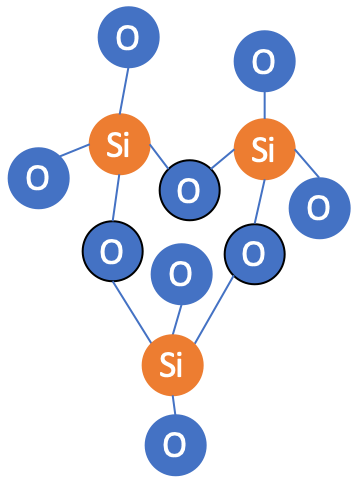
\includegraphics[width=.5\textwidth]{images/basic.png}
	\end{figure}
   \end{block}
   
   \column{0.3\textwidth}
   \begin{block}{Reduced Graph}
   \begin{itemize}
   \begin{footnotesize}
       \item V: Si atoms
       \item E: Bridging Oxygens
    \end{footnotesize}
   \end{itemize}
    \begin{figure}
	    \centering
        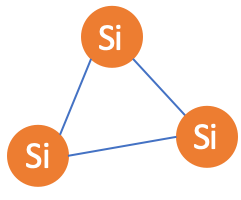
\includegraphics[width=.5\textwidth]{images/reduced.png}
	\end{figure}
   \end{block}
   
   \column{0.3\textwidth}
   \begin{block}{Topological Graph}
   \begin{itemize}
   \begin{footnotesize}
       \item V: Rings(closed paths)
       \item E: Bridging oxygen
    \end{footnotesize}
   \end{itemize}
    \begin{figure}
	    \centering
        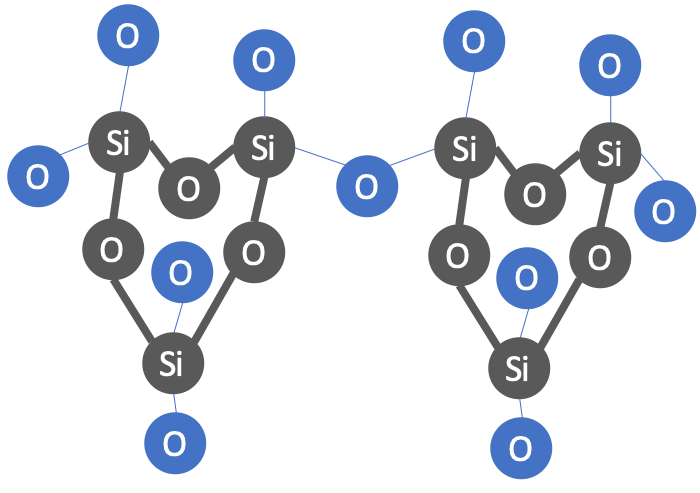
\includegraphics[width=.5\textwidth]{images/ring.png}
	\end{figure}   
   
   
   \end{block}
   
 \end{columns}
\end{frame}
%%%%%%%%%%%%%%%%%%%%%%%%%%%%%%%%%%%%%%%%%%%%%%%%%%%%%%%%%%%%%%%%%%%%%%%%%%%%%%%%%%%%%%%%%%%%%%%%%%%%%%%%%%
\frame{

\frametitle{Ground Truth}

\begin{minipage}[0.2\textheight]{\textwidth}
\begin{columns}[T]
    \begin{column}{0.5\textwidth}
    
    \begin{itemize}
    \begin{footnotesize}
    \item The ground truth is defined as whether or not an atom is part of a fracture at a certain time step.
    \item As the figure shows, some atoms are not highlighted in red, though they are on the fracture surface. So a K-nearest-neighbors algorithm will be applied to label those atoms.
    \end{footnotesize}  
    \end{itemize}
    \end{column}
    
    \begin{column}{0.5\textwidth}
    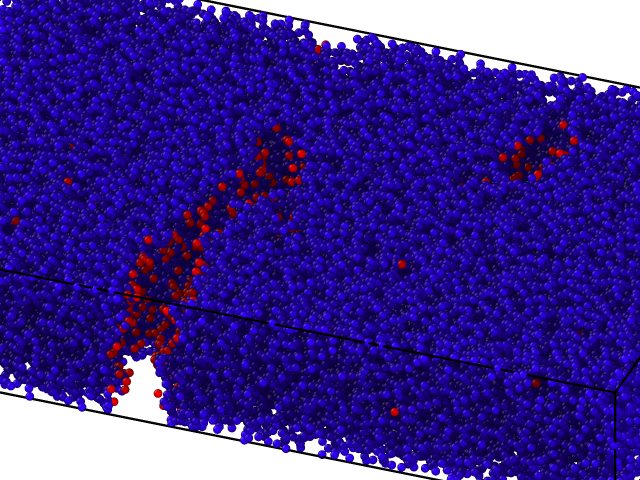
\includegraphics[width=5.5cm]{images/face.png}
    \end{column}
\end{columns}
\end{minipage}
}

%%%%%%%%%%%%%%%%%%%%%%%%%%%%%%%%%%%%%%%%%%%%%%%%%%%%%%%%%%%%%%%%%%%%%%%%%%%%%%%%%%%%%%%%%%%%%%%%%%%%%%%%%%
\frame
{
\frametitle{Voronoi Cell Volume}
\begin{block}{}
We also define the ground truth using a local density measure that we call the \textbf{Voronoi cell volume, $v_i$}, around a certain atom $i$. It is the empty space surrounding an atom.
\newline\newline
If $v_i$ exceeds a certain threshold, then the atom $i$ is defined as part of a nucleation event. Thus, $y_i = 1$.
\newline\newline
The threshold:
\centering $nuc_v = \frac{(v_i - \mu_v)}{\sigma_v}$
Thus, the ground truth can be defined as:
    \[
    y_i = \begin{cases}
      0 & \text{if }(nuc_v)_i \le 1 \\
      1 & \text{if }(nuc_v)_i > 1 \\
    \end{cases} 
    \]
\end{block}
}

%%%%%%%%%%%%%%%%%%%%%%%%%%%%%%%%%%%%%%%%%%%%%%%%%%%%%%%%%%%%%%%%%%%%%%%%%%%%%%%%%%%%%%%%%%%%%%%%%%%%%%%%%%
\frame
{
\frametitle{Example of 3D Fracture}
\begin{block}{}
    \begin{figure}[h]
			\centering
			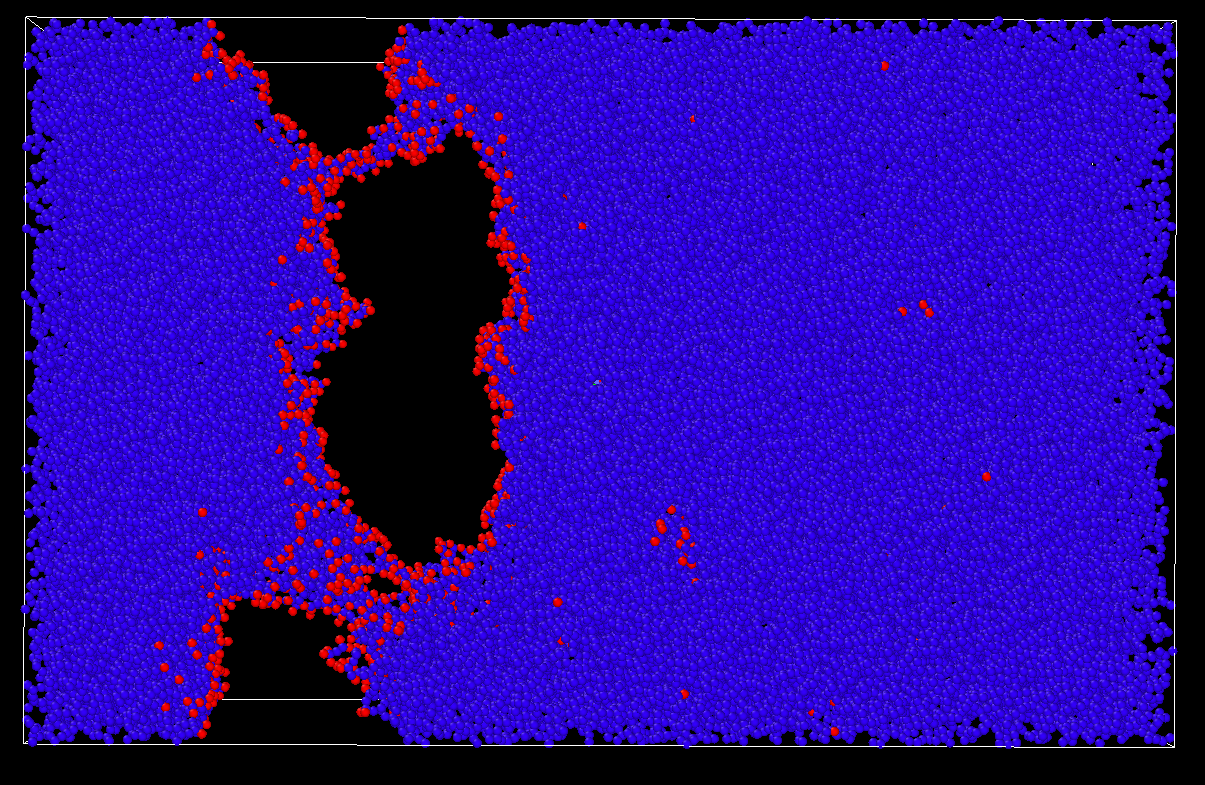
\includegraphics[width=.7\textwidth]{volcolor.png}
			\caption{Red atoms have a surrounding volume greater than the threshold}
    \end{figure}
\end{block}
}

%%%%%%%%%%%%%%%%%%%%%%%%%%%%%%%%%%%%%%%%%%%%%%%%%%%%%%%%%%%%%%%%%%%%%%%%%%%%%%%%%%%%%%%%%%%%%%%%%%%%%%%%%%

\subsection{Machine Learning Methods}
\frame{
\frametitle{Machine Learning Methods}

From the minutes

Features are an important part of this section

Physical features

Local topological features

Global topological features - read the SOW for an explanation of this , in section 5.2
}

%%%%%%%%%%%%%%%%%%%%%%%%%%%%%%%%%%%%%%%%%%%%%%%%%%%%%%%%%%%%%%%%%%%%%%%%%%%%%%%%%%%%%%%%%%%%%%%%%%%%%%%%%%
\frame{
\frametitle{Physical Features}
\begin{block}{}
Move Voroni Cell slide here. 
\end{block}

}
%%%%%%%%%%%%%%%%%%%%%%%%%%%%%%%%%%%%%%%%%%%%%%%%%%%%%%%%%%%%%%%%%%%%%%%%%%%%%%%%%%%%%%%%%%%%%%%%%%%%%%%%%%
\frame{
\frametitle{Local Topological Features}
\begin{block}{}
\textbf{Number of bridging oxygen:} These features include number of bonds an atom holds as well as the Qn structure where an Si atom is surrounded by n bridging O atoms, each forming an Si–O–Si group.
\end{block}

\begin{block}{}
k-th neighbor quantities. See SOW
\end{block}
}
%%%%%%%%%%%%%%%%%%%%%%%%%%%%%%%%%%%%%%%%%%%%%%%%%%%%%%%%%%%%%%%%%%%%%%%%%%%%%%%%%%%%%%%%%%%%%%%%%%%%%%%%%%
\frame{
\frametitle{Global Topological Features}

\begin{block}{}
\textbf{Centrality Measures:} By constructing a graph representation of the silicate glass, we will be able to compute centrality measures that give an idea on how important certain atoms, are relative to the rest of the network.
\end{block}
}
%%%%%%%%%%%%%%%%%%%%%%%%%%%%%%%%%%%%%%%%%%%%%%%%%%%%%%%%%%%%%%%%%%%%%%%%%%%%%%%%%%%%%%%%%%%%%%%%%%%%%%%%%%
\frame{
\frametitle{Machine Learning}

\begin{block}{}
Next few slides will be taken from the machine learning algorithm part of the SOW. 
\end{block}
}
%%%%%%%%%%%%%%%%%%%%%%%%%%%%%%%%%%%%%%%%%%%%%%%%%%%%%%%%%%%%%%%%%%%%%%%%%%%%%%%%%%%%%%%%%%%%%%%%%%%%%%%%%%







\frame{
\frametitle{See Demo video}
\begin{frame}
abc
\includemovie[poster,autoplay,externalviewer, text={\small(Loading failure.mp4)}]{6cm}{6cm}{failure.mp4}
% \includemedia
% [
%   activate=pageopen,
%   width=200pt,height=150pt,
%   addresource=bloch.mp4,
% %   text={\small(Loading bloch.mp4)}
%   flashvars={%
%      source=bloch.mp4% same path as in addresource!
%    &autoPlay=true%    % optional configuration
%    &loop=true%        % variables
%   } 
%   ]{}{VPlayer.swf}

  def

%%%%%%%%%%%%%%%%%%%%%%%%%%%%%%%%%%%%%%%%%%%%%%%%%%%%%%%%%%%%%%%%%%%%%%%%%%%%%%%%%%%%%%%%%%%%%%%%%%%%%%%%%%


\end{frame} }






%%%%%%%%%%%%%%%%%%%%%%%%%%%%%%%%%%%%%%%%%%%%%%%%%%%%%%%%%%%%%%%%%%%%%%%%%%%%%%%%%%%%%%%%%%%%%%%%%%%%%%%%%%


